\begin{center}
    \renewcommand{\nextTitle}{ГЛАВА 3. SLAM-АЛГАРЫТМЫ}
    \addcontentsline{toc}{section}{\nextTitle}
    \section*{\nextTitle}
\end{center}

\vspace{5mm}

\renewcommand{\cursection}{3}
\setcounter{figure}{0}

\renewcommand{\nextTitle}{3.1 Асноўныя звесткі}
\addcontentsline{toc}{subsection}{\nextTitle}
\subsection*{\nextTitle}

\vspace{5mm}

Задача адначасовай лакалізацыі і пошуку на мапе (англ. \textit{Simultaneous Localization and Mapping, SLAM})
спалучае ў сабе выкарыстанне разнастайных датчыкаў (лазерныя сканеры, RGB альбо RGB-D
камеры і іншае) з мэтай ацэнкі пазіцыі робата/БПЛА ў прасторы і адначасовай пабудовы мапы мясцовасці.
Задача фармулюецца як для двухмерных, так і для трохмерных асяроддзяў: нас цікавіць
трохмерная задача, тым больш што двухмерная версія задачы лічыцца вырашанай. З адначасовасці
пабудовы мапы і ацэнкі пазіцыі ў прасторы вынікае патрабаванне да алгарытма працаваць у рэальным часе,
што накладае асаблівыя патрабаванні да алгарытмаў і абсталявання, на якім алгарытмы запускаюцца.

Сваё найбольшае развіццё рашэнне SLAM задачы атрымала ў апошнія дзесяцігоддзі. Даследванне
задачы можна ўмоўна падзяліць на тры этапы (прапанаваныя ў \cite{DBLP:journals/corr/CadenaCCLSN0L16},
\cite{Li2016RealtimeSL}). Першы перыяд, прыблізна 1986-2004, можна назваць ``класічным''.
У гэтыя часы асноўным накірункам працы па рашэнні задачы была імавернасная фармуліроўка
і падыходы, заснаваныя на фільтрах. У другі перыяд, 2004-2015, былі даследаваныя асноўныя
ўласцівасці, такія як назіральнасць, збежнасць і ўзгодненасць алгарытмаў. У гэты час былі
праведзеныя цесныя аналогія з існуючымі падыходамі ў галіне камп'ютарнага зроку,
была ствароная вялікая колькасць рэалізацыяў з адкрытым зыходным кодам, з'яўляліся першыя спробы
прымянення SLAM у практычных прыкладаннях.

Мяркуецца, што на трэці этап распрацоўка перайшла зусім нядаўна, у апошнія гады: гэта звязваюць
з публікацыямі такіх алгарытмаў, як ORB-SLAM ці LSD-SLAM, якія па сваёй
функцыянальнасці моцна пераўзыходзяць любыя ранейшыя публікацыі. Прынцыпы працы гэтых алгарытмаў,
як і некаторых іншых, будуць разгледжаныя далей.

Важна успрымаць SLAM не як адзіны прапанаваны алгарытм, але як канцэпцыю. SLAM-сістэмы складаюцца са
шматлікіх частак і кожная з гэтых частак можа ўдзельнічаць у рашэнні агульнай задачы з той ці іншай эфектыўнасцю.

Для задачы рэканструкцыі паверхні SLAM-сістэма наўрад ці будзе
аптымальным рашэннем: пабудова шчыльных мадэляў у рэальным часе пакуль яшчэ застаецца
слаба вырашанай задачай. Тут і далей SLAM-сістэмы нас цікавяць сваімі выхаднымі
дадзенымі: пасля апрацоўкі дадзеных у рэальным часе захаваныя пазіцыі, павароты камераў
у часе і пабудаваная глабальная мапа могуць быць эфектыўна выкарыстаныя ў якасці
ўваходных дадзеных афлайн алгарытма, падвышаючы ягоную дасканаласць і хуткасць працы.

Як вынікае з назвы, алгарытмы рашаюць дзве асноўныя задачы: лакалізацыю і пошук на мапе.
На першых этапах даследавання задачы разглядаліся асобна, але з цягам часу стала зразумела,
што задачы цесна звязаныя паміж сабой і рашэнне адной з іх моцна дапамагае ў рашэнні іншай. Мапа патрэбная для
эфектыўнага пошуку пазіцыі ў прасторы, у той жа час з ацэнкай становішча мапа сабірае больш дадзеных
і становіцца больш дакладнай.

Большасці сучасных SLAM-алгарытмаў прысутная магчымасць замыкаць цыклы (\textit{loop closure}) -
знаходзіць аб'екты, якія сустракаліся ў прасторы раней у межах таго ж пралёту/праходу асяроддзя,
распазнаваць іх у якасці \textit{знаёмых} і глабальна ўдасканальваць мапу на падставе факта
паўторна сустрэнутага аб'екта. Падыход добра паўплываў на якасць працы мноства алгарытмаў
і зарэкамендаваў сябе адпаведным чынам -- прычына поспеху ў надзейнасці вонкавых сістэм, здольных
успрымаць відэаплыню і знаходзіць аб'екты незалежна ад асноўных плыняў алгарытма.

Разгледзім асноўныя этапы падрабязней.

\renewcommand{\nextTitle}{3.2 Ключавыя паняцці і падыходы}
\addcontentsline{toc}{subsection}{\nextTitle}
\subsection*{\nextTitle}

\vspace{5mm}

\renewcommand{\nextTitle}{3.2.1 Лакалізацыя}
\addcontentsline{toc}{subsubsection}{\nextTitle}
\subsubsection*{\nextTitle}

Пры руху пазіцыя БПЛА ў дыскрэтным часе задаецца матрыцай $T \in \mathbb{R}^{4\times4}$.
Паслядоўнасць такіх матрыцаў -- траекторыя пралёту. Лакалізацыя - пошук такой матрыцы ў вызначаны момант часу.
Для адкрытых прастораў задача была часткова вырашаная з запускам GPS - глабальнай сістэмы
пазіцыянавання; у прасторах, дзе GPS недаступны, таксама можа выкарыстоўвацца вонкавае
абсталявання для лакалізацыі, што часта з'яўляецца непрактычным альбо дарагім рашэннем.
Выкарыстанне датчыкаў, усталяваных на БПЛА, для лакалізацыі ў прасторы, робіць падыходы
да рашэння задачы больш універсальнымі. Лакалізацыю з дапамогай толькі камераў часам
таксама называюць візуальнай адаметрыяй (англ. \textit{Visual Odometry}). Надзейныя механізмы
лакалізацыі аўтаномных БПЛА асабліва важныя праз знаходжанне БПЛА ў паветры і
немагчымасць спыніцца, у адрозненні на наземных робатаў.

\renewcommand{\nextTitle}{3.2.2 Пошук на мапе}
\addcontentsline{toc}{subsubsection}{\nextTitle}
\subsubsection*{\nextTitle}

Ёсць некалькі важных аспектаў пабудовы мапы. Па-першае, мапа выкарыстоўваецца для пракладкі
маршрутаў і лакалізацыі перашкодаў -- асноўныя элементы для аўтаномнай навігацыі. Па-другое --
мапа на выхадзе можа быць цікавая сама па сабе: яна можа пасля выкарыстоўвацца для візуалізацыі пралёта
па мясцовасці альбо як уваходныя дадзеныя для алгарытмаў афлайн-рэканструкцыі, для распазнавання
аб'ектаў і гэтак далей. Трэці і, магчыма, самы важны аспект у дачыненні да канцэпцыі SLAM --
добра пабудаваная мапа дазваляе лакалізаваць БПЛА ў прасторы.

Адзін з важных аспектаў пошука на мапе -- магчымасць пошуку элементаў, месцаў,
якія былі наведаныя і пабачаныя раней.
Гэты працэс называецца \textit{замкненнем цыклаў} (англ. \textit{loop closure}).

\vspace{5mm}

Такім чынам, лакалізацыя і пошук на мапе не выступаюць як дзве асобныя і незалежныя
часткі алгарытма, але дапаўняюць і паляпшаюць адна адну. Пошук сябе на папярэдне пабудаванай мапе
(напрыклад, пры паўторным пралёце той жа мясцовасці) дазваляе лакалізаваць БПЛА з
якасцю, параўнальнай з якасцю пабудаванай мапы, у сваю чаргу лакалізацыя пры дапамозе
адаметрыі і старонніх датчыкаў паслядоўна ўдасканальвае мапу. Сфармуляваўшы гэтую залежнасць
іншымі словамі, пры наяўнасці дакладна вырашанай задачы альбо лакалізацыі, альбо пошуку на мапе,
іншая задача таксама можа лічыцца вырашанай.

\renewcommand{\nextTitle}{3.3 Падыходы да рэалізацыі}
\addcontentsline{toc}{subsection}{\nextTitle}
\subsection*{\nextTitle}

\vspace{5mm}

Як зазначаецца ў \cite{Li2016RealtimeSL}, архітэктура любой SLAM-сістэмы
можа быць прадстаўленая схемай з малюнку \cursection.\ref{fig:slam-architecture}. Фронтэнд выконвае
першасную апрацоўку дадзеных, якія паступаюць са знешніх датчыкаў. Для алгарытмаў,
заснаваных на пошуку асаблівых кропак, фронтэнд займаецца іх пошукам і апісаннем;
для алгарытмаў, якія працуюць непасрэдна са значэннямі пікселяў, выконваецца трэкінг паміж
кадрамі. Усе вынікі першаснай апрацоўкі пасля перадаюцца бэкэнду.

Бэкэнд, у сваю чаргу, займаецца пабудовай графа залежнасцяў, аптымізацыяй на графе.
Можна сказаць, што сёння асноўныя намаганні даследчыкаў прыкладаюцца да фронтэнду; бэкэнд
жа можна ўмоўна лічыць стандартаваным, яго задача -- аптымізацыя графа, які змяшчае інфармацыю
пра пазіцыі ключавых кадраў і залежнасці паміж імі.

Задача SLAM з выкарыстаннем адзінай камеры ў якасці сэнсара на сённяшні момант
лічыцца нявырашанай па прычыне нястачы вылічальных магутнасцяў, недахопе дадзеных
пра глыбіню выявы і складанасці пошуку і асацыяцыі паміж сабой ключавых кропак.
У некаторых сітуацыях некаторыя з вышэйзгаданых праблемаў могуць быць вырашаныя
(альбо часткова вырашаныя). Напрыклад, задача высвятлення глыбіні выявы не стаіць так
востра пры выкарыстанні стэрэакамеры, альбо калі пра манакулярную камеру вядома,
што яна глядзіць уніз (англ. \textit{downward looking camera}).

Важным крокам у рэалізацыі SLAM-алгарытмаў стала дамінаванне ідэі раздзялення лакалізацыі
і пошуку на мапе ў асобныя плыні. Упершыню практычнае прымяненне ідэя знайшла
ў сістэме PTAM (\textit{Parallel Tracking and Mapping for Small AR Workspaces}, \cite{Klein:2007:PTM:1514339.1514363}).
Лакалізацыйная плыня PTAM займаецца пошукам адпаведнасцяў у дадзеных і запускае
аптымізацыю па рухах камеры. У гэты ж час плыня з мапай калекцыянуе вынікі лакалізацыі,
трыангулюе выяўленыя асаблівасці ў трохмерныя кропкі і абнаўляе глабальную мапу.
Са з'яўленнем такога падыходу сталі відавочнымі ягоныя перавагі і амаль кожная
сучасная SLAM-сістэма пабудаваная па падобным прынцыпе.

\begin{figure}[H]
  \centering
  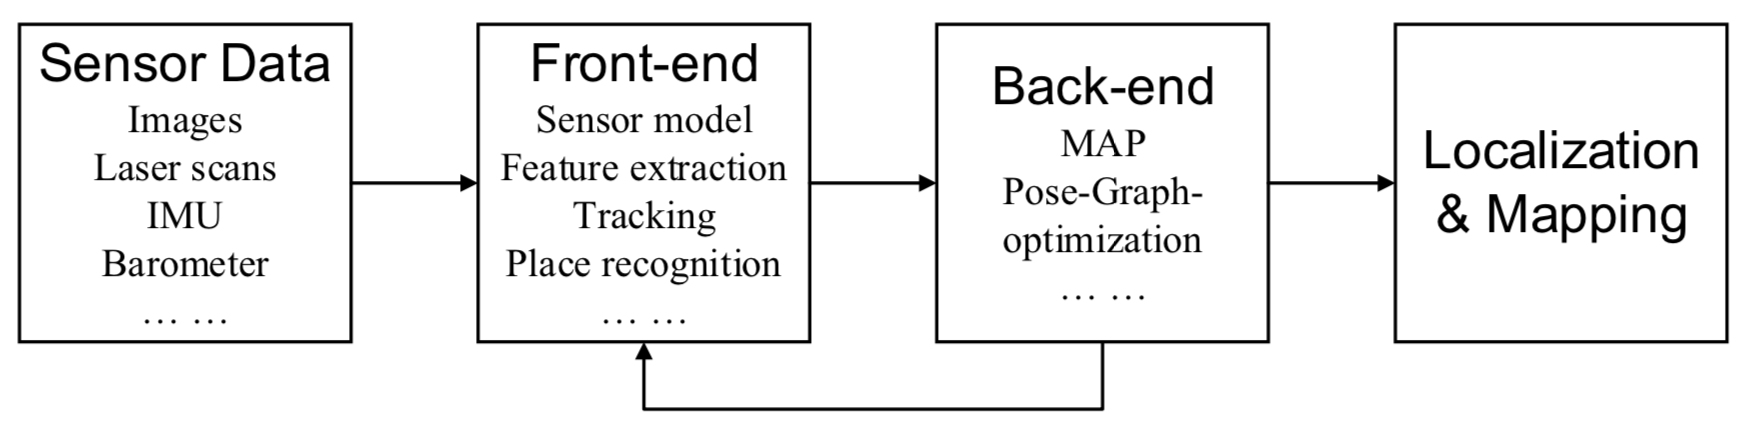
\includegraphics[width=.9\textwidth]{slam-architecture}
  \captionsetup{labelformat=empty}
  \caption{Малюнак \cursection.\arabic{figure}: высокаўзрозневая архітэктура SLAM-алгарытмаў}
  \label{fig:slam-architecture}
\end{figure}

\renewcommand{\nextTitle}{3.4 Агляд SLAM-сістэм}
\addcontentsline{toc}{subsection}{\nextTitle}
\subsection*{\nextTitle}

Далей ідзе апісанне асаблівасцяў некаторых SLAM-сістэм, якія на сённяшні дзень паказваюць найлепшыя вынікі.
Некаторыя з іх заснаваныя на пошуку асаблівых кропак (\textit{feature-based SLAM}),
другія -- на простых метадах (\textit{direct SLAM}), трэція -- камбінуюць у сабе
абодва падыхода (\textit{semi-direct SLAM}).
Да прыкладу, ORB-SLAM (\cite{murTRO2015}, \cite{murORB2}) адносіцца да першай катэгорыі
SLAM-сістэм, LSD-SLAM (\cite{engel14eccv}) -- да другой, SVO(\cite{Forster2014ICRA}) --
да трэцяй.

\renewcommand{\nextTitle}{3.4.1 ORB-SLAM}
\addcontentsline{toc}{subsubsection}{\nextTitle}
\subsubsection*{\nextTitle}

ORB-SLAM (\cite{murTRO2015}, \cite{murORB2}) -- манакулярная SLAM-сістэма,
заснаваная на пошуку асаблівасцяў на выявах (\textit{feature-based}),
спраектаваная для працы ў маленькіх і вялікіх, замкнёных і адкрытых прасторах.

Асноўныя асаблівасці:

\begin{itemize}
  \item выкарыстанне адных і тых жа ключавых кропак на ўсіх этапах працы алгарытма;
  \item чатыры асноўныя задачы, якія адначасова рашае алгарытм: трэкінг (\textit{tracking}),
  нанясенне дадзеных на мапу (\textit{mapping}), рэлакалізацыя (\textit{relocalization}),
  замкненне цыклаў (\textit{loop closing});
  \item неабмежаваны рост памераў мапы \textit{толькі} з ростам аглядаемай тэрыторыі;
  \item выкарыстанне ORB-дэскрыптараў як найлепшых па хуткасці (без ужывання GPU)
  і інварыянтнасці да зменаў у павароце і асвятленні;
  \item хуткі трэкінг і пошук на мапе на лакальных абласцях бачнасці, што дасягаецца
  праз выкарыстанне \textit{графа узаемабачнасці} (\textit{covisibility graph});
  \item новы аўтаматычны і надзейны спосаб ініцыялізацыі, які стварае пачатковыя мапы
  як для планарных, так і для непланарных паверхняў;
  \item пазбаўленне ад лішніх ключавых кадраў па стратэгіі ``выжывання наймацнейшага''
  (\textit{survival of the fittest});

  \begin{figure}[H]
    \centering
    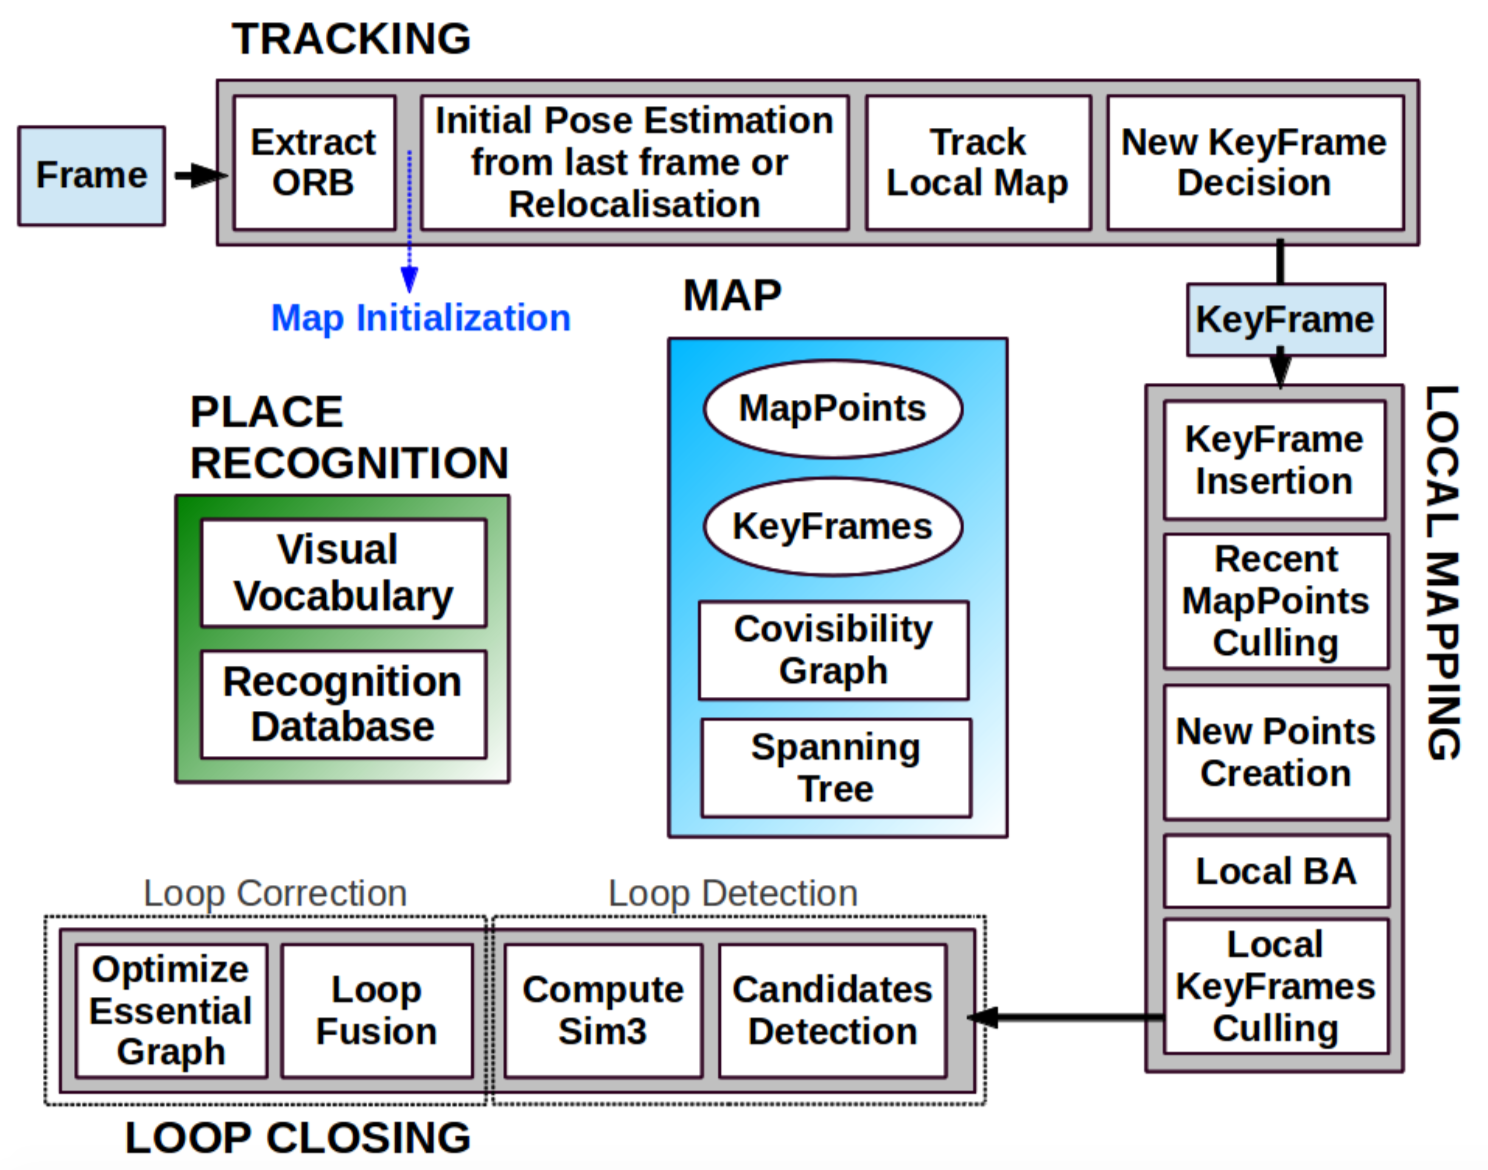
\includegraphics[width=.7\textwidth]{orb-architecture}
    \captionsetup{labelformat=empty}
    \caption{Малюнак \cursection.\arabic{figure}: архітэктура ORB-SLAM}
    \label{fig:orb-architecture}
  \end{figure}

  \item агульная схема працы алгарытма прадстаўленая на малюнку \cursection.\ref{fig:orb-architecture}.
\end{itemize}

Арыгінальная публікацыя (\cite{murTRO2015}) прыводзіла апісанне манакулярнай сістэмы,
у другой рэдакцыі алгарытма (ORB-SLAM2, \cite{murORB2}) дадалася падтрымка стэрэа і RGB-D камер.
Пра рэалізацыю варта зазначыць, што першая версія была даступная толькі пад ROS
(аперацыйная сістэма, шырока распаўсюджаная сярод робататэхнікаў),
у сваю чаргу ў другой версіі з'явіліся ўласныя сродкі візуалізацыі, здольныя працаваць незалежна.

\renewcommand{\nextTitle}{3.4.2 LSD-SLAM}
\addcontentsline{toc}{subsubsection}{\nextTitle}
\subsubsection*{\nextTitle}

У адрозненні ад разгледжанай вышэй сістэмы ORB-SLAM, заснаванай на пошуку
асаблівых кропак, LSD-SLAM (\cite{engel14eccv}) выкарыстоўвае \textit{простыя} (\textit{direct})
падыходы да працы з выявамі, то бок працуе непасрэдна са значэннямі ў пікселях.

\begin{figure}[H]
  \centering
  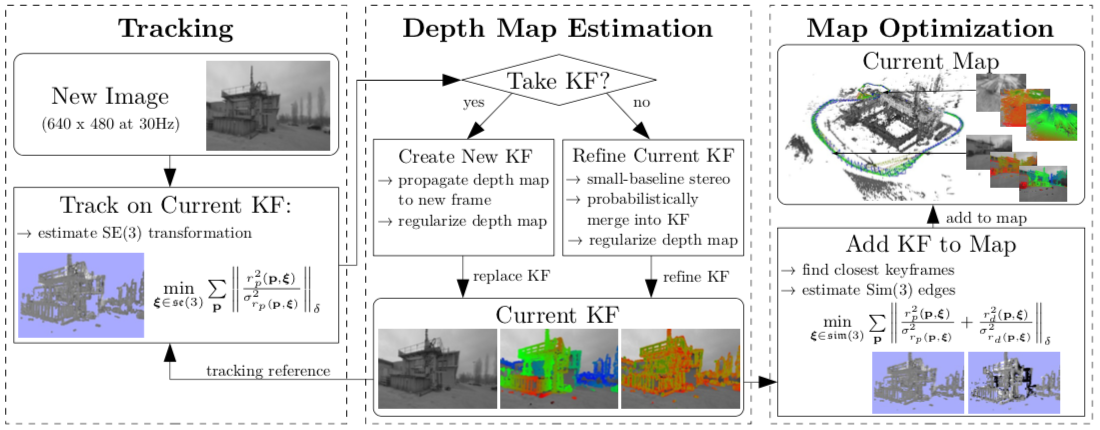
\includegraphics[width=.8\textwidth]{lsd-architecture}
  \captionsetup{labelformat=empty}
  \caption{Малюнак \cursection.\arabic{figure}: архітэктура LSD-SLAM}
  \label{fig:lsd-architecture}
\end{figure}

\begin{itemize}
  \item працуе ў рэальным часе на CPU;
  \item складаецца з трох асноўных кампанент: трэкінг, падлік набліжэння для мапы
  глыбіняў і аптымізацыя мапы;
  \item трэкінг кампанента паслядоўна апрацоўвае новыя здымкі, прымаючы да ўвагі
  папярэдні і бягучы ключавыя здымкі;
  \item другая кампанента выкарыстоўвае здымкі каб альбо палепшыць, альбо замяніць
  бягучы ключавы кадр і ацэньвае глыбіню сцэны простымі (\textit{direct})
  і імавернаснымі падыходамі;
  \item здымкі, якія канчаткова пазначаныя як ключавыя (мапа глыбіняў больш
  змяняцца не будзе) заносяцца на глабальную мапу;
  \item мапа - граф узаемаразмяшчэння ключавых кадраў. Паколькі алгарытм таксама
  ацэньвае мапы глыбіняў, то мапа, па сутнасці, ўяўляе сабой напаўшчыльную
  трохмерную рэканструкцыю паверхні;
  \item аўтары ініцыялізуюць першы ключавы кадр \textit{выпадковай} мапай глыбіняў
  з вялікімі перападамі. Сцвярджаецца, што пры значных рухах камеры ў прасторы
  ў першую секунду, першасная мапа глыбіняў будзе хутка збягацца. Аўтары прызнаюцца
  ў неабходнасці дапрацаваць гэтую частку сістэмы; пры тэставых запусках мапа
  глыбіняў для ініцыялізацыі бралася непасрэдна з датасэтаў (то бок была дакладна
  вядомая), на практыцы падобны падыход можа запатрабаваць пэўнага чалавечага ўдзелу;
  \item архітэктура сістэмы прадстаўленая на малюнку \cursection.\ref{fig:lsd-architecture}.
\end{itemize}

\renewcommand{\nextTitle}{3.4.3 SVO}
\addcontentsline{toc}{subsubsection}{\nextTitle}
\subsubsection*{\nextTitle}

У адрозненні ад папярэдніх двух прыкладаў, SVO (\textit{Semi-Direct Monocular Visual Odometry},
\cite{Forster2014ICRA}) спалучае ў сабе як пошук і апісанне ключавых кропак, так і
простыя метады, праз што і атрымаў сваю назву (\textit{Semi-Direct, паўпросты}).

\begin{figure}[H]
  \centering
  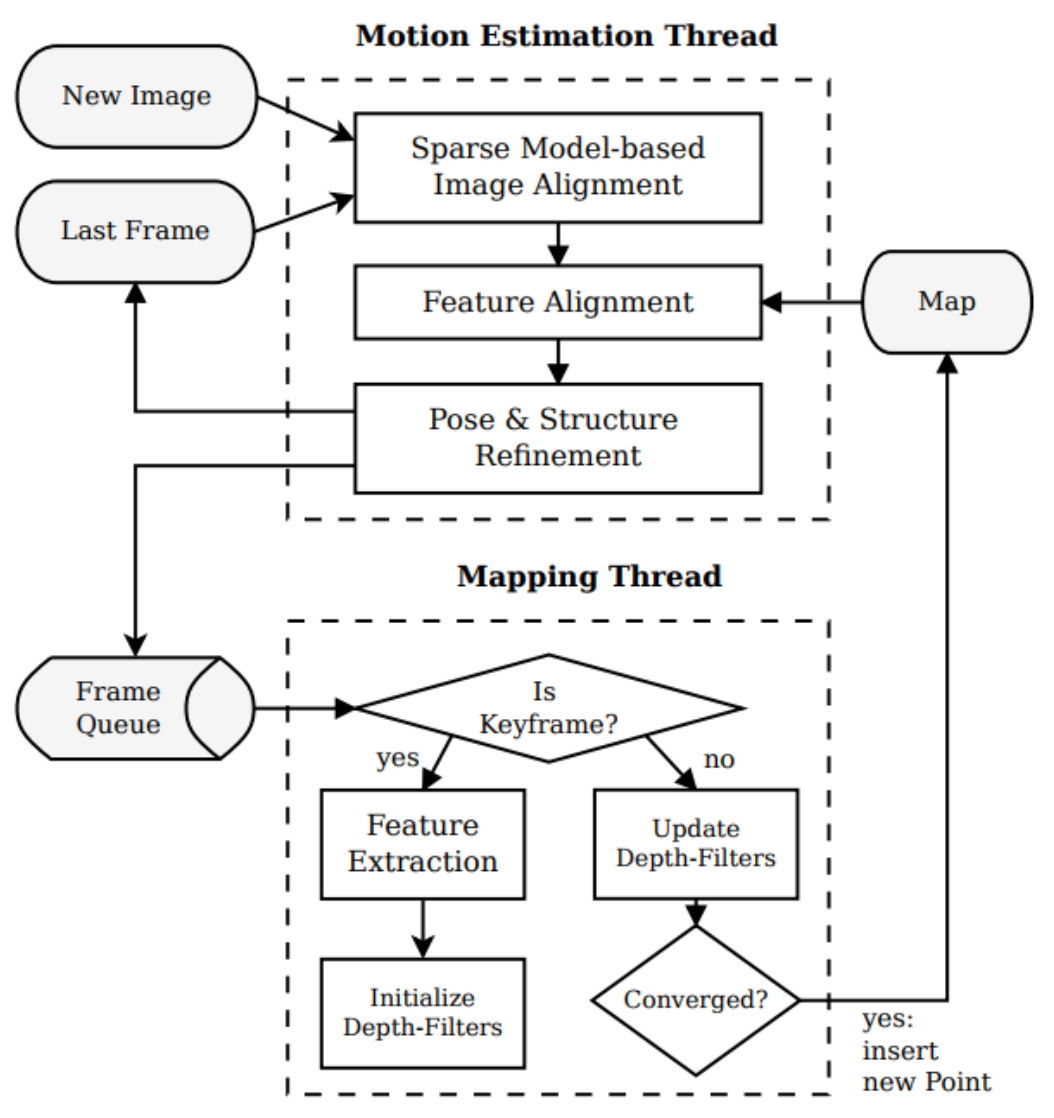
\includegraphics[width=.5\textwidth]{svo-architecture}
  \captionsetup{labelformat=empty}
  \caption{Малюнак \cursection.\arabic{figure}: архітэктура SVO}
  \label{fig:svo-architecture}
\end{figure}

\begin{itemize}
  \item спалучае ў сабе лепшае ад метадаў, заснаваных на ключавых кропках (выбар
  ключавых кадраў, сачэнне за мноствам кропак, паралельны трэкінг і пошук на мапе),
  і ад простых метадаў (хуткасць і дакладнасць);
  \item пошук адпаведнасцяў паміж ключавымі кропкамі здзяйсняецца няяўна як вынік
  прымянення простых метадаў (а не, напрыклад, matching-а);
  \item выманне ключавых кропак здзяйсняецца толькі на ключавых кадрах;
  \item пасля таго, як адпаведнасці паміж ключавымі кропкамі, а таксама пачатковая пазіцыя
  камеры ўсталяваныя, алгарытм толькі працуе з непасрэднымі значэннямі пікселяў у кропках.
  Пазіцыя камеры адносна папярэдняга кадра падлічваецца праз мінімізацыю фотаметрычнай памылкі;
  \item трохмерная кропка дадаецца на мапу толькі ў выпадку збежнасці адпаведнага
  фільтра глыбіняў, што азначае патрэбнасць у шматлікіх вымярэннях для кожнай асобнай кропкі;
  \item глыбінныя фільтры для ключавых кадраў ініцыялізуюцца сярэднім значэннем
  сярод усіх глыбінных фільтраў сцэны;
  \item свядзенне да мінімума выкідаў у вымярэннях;
  \item архітэктура сістэмы прадстаўленая на малюнку \cursection.\ref{fig:svo-architecture}.
\end{itemize}

\renewcommand{\nextTitle}{3.4.4 CNN-SLAM}
\addcontentsline{toc}{subsubsection}{\nextTitle}
\subsubsection*{\nextTitle}

Аўтары алгарытма CNN-SLAM \cite{DBLP:journals/corr/TatenoTLN17} прапаноўваюць альтэрнатыўны падыход да ацэнкі
глыбіні сцэны пры наяўнасці адзінай камеры. Найбольш класічным ў такім выпадку лічыцца
імітацыя стэрэакамеры (ацэнка глыбіні сцэны пра невялікіх рухах камеры ў прасторы), аднак такі
падыход мае пэўныя праблемы, якія не дазваляюць ягонае надзейнае выкарыстанне. Напрыклад,
падыход не прымяняльны пры паваротах у прасторы. Аўтары прапаноўваюць будаваць глыбіню,
базуючыся на адзіным кадры з дапамогай канвалюцыйных нейронных сетак
(\textit{Convolutional Neural Networks, CNN}, адсюль паходзіць назва алгарытма).
Сярод іншых асаблівасцяў алгарытма:

\begin{itemize}
    \item дазваляе абысці адно з найвялікшых абмежаванняў усіх SLAM-алгарытмаў --
    немагчымасць ацаніць рэальныя масштабы сцэны, якая аглядаецца. SLAM-алгарытмы
    заўжды даюць вынікі з дакладнасцю да масштабу, калі толькі не прымяняюцца спецыяльныя падыходы,
    якія дапамагаюць зразумець рэальныя памеры аб'ектаў. Прыкладам такога падыхода
    можа быць распазнаванне аб'ектаў і наступнае параўнанне з базай аб'ектаў,
    для якіх вядомыя іх фізічныя характарыстыкі. Зразумела, што такі падыход не дасць аніякіх
    вынікаў пры адсутнасці на сцэне хаця б аднаго аб'екта з базы;
    \item нейронная сетка навучаецца не на прыкладах з аднаго канкрэтнага асяроддзя,
    але па наборы дадзеных, які змяшчае ў сабе вельмі разнастайныя выявы. Гэта дазваляе,
    аднойчы навучыўшы SLAM-сістэму, запускаць яе ў разнастайных асяроддзях (у тым ліку --
    у незнаёмых) з аднолькавай паспяховасцю;
    \item мапы глыбіняў, згенераваныя нейроннай сеткай, хаця і глабальна карэктныя,
    даюць размытасці на вуглах, граніцах. Гэта не дазваляе выкарыстоўваць згенераваныя
    мапы глыбіняў у сваім пачатковым выглядзе, але дазваляе паспяхова выкарыстоўваць іх
    у якасці апрыорных ацэнак;
    \item мапы глыбіняў, хоць і з размытасцямі, але даюць уяўлянне пра сапраўдную
    глыбіню сцэны, яе масштаб;
    \item мапы глыбіняў не трапляюць пад уплыў праблемаў з паваротамі камераў у прасторы
    (без адпаведнага перасоўвання ў прасторы), праз што трэкінг становіцца значна больш надзейным;
    \item наяўнасць працэса нармалізацыі для ўзгаднення памераў і каляровых характарыстыкаў
    выяваў паміж наборамі, на якіх алгарытм вучыўся, і выявамі, якія паступаюць падчас працы алгарытма;
    \item для падтрымкі працы ў рэальным часе глыбіня ацэньваецца толькі для ключавых кадраў,
    а не для ўсіх, якія паступаюць з відэаплыні;

    \begin{figure}[H]
      \centering
      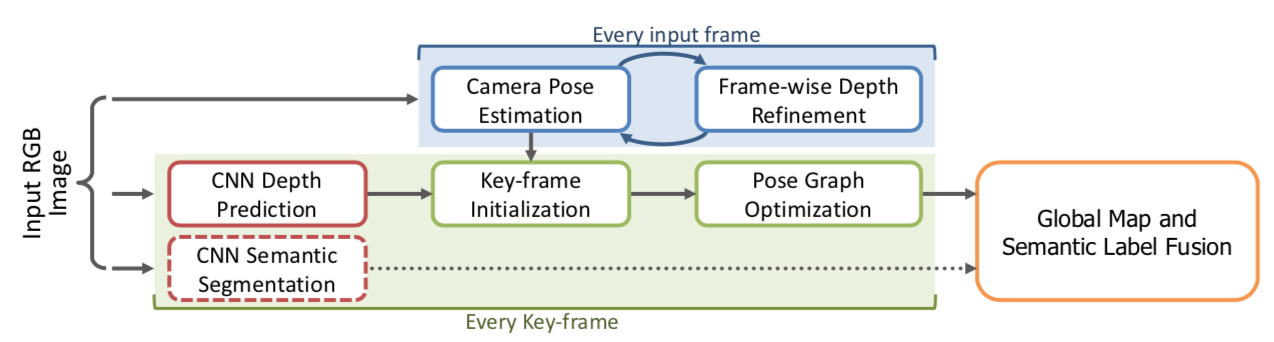
\includegraphics[width=.9\textwidth]{cnn-architecture}
      \captionsetup{labelformat=empty}
      \caption{Малюнак \cursection.\arabic{figure}: архітэктура CNN-SLAM}
      \label{fig:cnn-architecture}
    \end{figure}

    \item дадатковая нейронная сетка для семантычнай сегментацыі выяваў -- асобнае даследаванне,
    праведзенае ў межах працы і рэалізаванае ў тым жа фрэймворку;
    \item вынікі эксперыментаў паказваюць, што алгарытм на большасці набораў дадзеных працуе
    хутчэй за LSD-SLAM і ORB-SLAM, сённяшніх лідэраў сярод SLAM-алгарытмаў,
    з якімі праводзілася параўнанне, а таксама дае непараўнальна лепшую ацэнку для глыбіні сцэны;
    \item апроч таго, былі праведзеныя асобныя эксперыменты па прымяняльнасці алгарытма да
    дадзеных, якія атрымліваліся толькі праз павароты камеры. Паколькі гэтая папулярная сярод
    SLAM-сістэмаў праблема ў выпадку з CNN-SLAM абыходзіцца праз выкарыстанне нейронных сетак
    для ацэнкі глыбіні, то, як вынік, алгарытм паказвае дастойныя вынікі на такога кшталту дадзеных
    і моцна апярэджвае любыя іншыя сучасныя алгарытмы;
    \item архітэктура сістэмы прадстаўленая на малюнку \cursection.\ref{fig:cnn-architecture}.
\end{itemize}

\newpage
